\documentclass[12pt,letterpaper]{exam}
\usepackage[lmargin=1in,rmargin=1in,tmargin=1in,bmargin=1in]{geometry}
\usepackage{../style/exams}

% -------------------
% Course & Exam Information
% -------------------
\newcommand{\course}{MAT 108: Exam 2}
\renewcommand{\term}{Spring -- 2023}
\newcommand{\examdate}{04/03/2023}
\newcommand{\timelimit}{85 Minutes}

\setbool{hideans}{false} % Student: True; Instructor: False

% -------------------
% Content
% -------------------
\begin{document}

\examtitle
\instructions{Write your name on the appropriate line on the exam cover sheet. This exam contains \numpages\ pages (including this cover page) and \numquestions\ questions. Check that you have every page of the exam. Answer the questions in the spaces provided on the question sheets. Be sure to answer every part of each question and show all your work. If you run out of room for an answer, continue on the back of the page --- being sure to indicate the problem number.} 
\scores
\bottomline
\newpage

% ---------
% Questions
% ---------
\begin{questions}

% Question 1
\newpage
\question[15] A sports analyst is testing the claim whether taller basketball players are inherently better than shorter players. The analyst creates a linear regression to predict the number of baskets scored in 60~seconds by players between 75~in and 86~in. The model is found to be $\widehat{y}= 1.2x - 69.7$ with $r= 0.8691$. 
	\begin{enumerate}[(a)]
	\item Predict the number of shots made in the given time by a player with a height of 78~in. \pvspace{0.1cm}
		\[
		\widehat{y}(78)= 1.2(78) - 69.7= 93.6 - 69.7= 23.9 \text{ shots}
		\] \pspace
	
	\item Which of the following scatterplots is the most likely to represent the data and the model? \par
		\begin{figure}[!ht]
		\centering
		\hfill
		\begin{subfigure}[b]{0.3\textwidth}
		\includegraphics[width=\textwidth]{plot1.png}
		\caption{}
		\end{subfigure}
		\hfill
		\begin{subfigure}[b]{0.3\textwidth}
		\includegraphics[width=\textwidth]{{plot2.png}}
		\caption{}
		\end{subfigure} \par
		\hfill
		\begin{subfigure}[b]{0.3\textwidth}
		\includegraphics[width=\textwidth]{{plot3.png}}
		\caption{\cmark}
		\end{subfigure}
		\hfill
		\begin{subfigure}[b]{0.3\textwidth}
		\includegraphics[width=\textwidth]{{plot4.png}}
		\caption{}
		\end{subfigure}
		\end{figure} 
		
	{\itshape Because $r= 0.8691 > 0$ or because $b_1= 1.2 > 0$, we know the slope of the model is positive. This leaves only (a) or (c) as options. As $r= 0.8691$ indicates a regression where the line fits the data points `slightly well', (c) is more likely than (a). Therefore, (c) is the most likely scatterplot.}
	
	\item Find the value of the coefficient of determination. \pspace
		\[
		\text{Coeff. of Determ.}= r^2= (0.8691)^2= 0.7553
		\] \pvspace{0.8cm}
	
	\item Should one use this model to predict the shots made by someone with a height of 65~in?	\pspace
	
	{\itshape One should not use the model to make a prediction in this case. A height of 65~in is `far' outside the range of 75~in to 85~in players used to create the model. This `extreme' extrapolation may lead to an unreliable result.}
	\end{enumerate}



% Question 2
\newpage
\question[10] An administrator is trying to determine if there is any correlation between student success and a new support program offered by the college. They gather the following data:
	\begin{table}[!ht]
	\centering
	\begin{tabular}{|l||c|c|c|} \hline
	& Program Participant & Non-Participant & Total \\ \hline \hline
	Graduated & 87 & 453 & 540 \\ \hline
	Not Graduated & 13 & 187 & 200 \\ \hline \hline
	Total & 100 & 640 & 740 \\ \hline
	\end{tabular}
	\end{table}

\begin{enumerate}[(a)]
\item Find the probability that a randomly selected student was a program participant and graduated.
\item Find the probability that a randomly selected student participated in the program or graduated. 
\item Find the probability that a randomly selected program participant graduated. 
\end{enumerate} \pspace

{\itshape
\sol  
\begin{enumerate}[(a)]
\item 
	\[
	P(\text{Participant and Graduated})= \dfrac{87}{740} \approx 0.117568
	\] \pspace

\item 
	\[
	\begin{aligned}
	\hspace{-1cm} P(\text{Participant or Graduated})&= P(\text{Participant}) + P(\text{Graduated}) - P(\text{Participant and Graduated}) \\[0.3cm]
	\hspace{-1cm}&= \dfrac{100}{740} + \dfrac{540}{740} - \dfrac{87}{740} \\[0.3cm]
	\hspace{-1cm}&= \dfrac{553}{740} \approx 0.747297
	\end{aligned}
	\]  \pvspace{0.1cm}
	\[ \text{\itshape OR} \] \pvspace{0.1cm}
	\[
	P(\text{Participant or Graduated})= \dfrac{87 + 453 + 13}{740}= \dfrac{553}{740} \approx 0.747297
	\] \pspace

\item 
	\[
	P(\text{Graduated} \;|\; \text{Participant})= \dfrac{P(\text{Graduated and Participant})}{P(\text{Participant})}= \dfrac{87/740}{100/740}= \dfrac{87}{100}= 0.87
	\] \pvspace{0.1cm}
	\[ \text{\itshape OR} \] \pvspace{0.1cm}
	\[
	P(\text{Graduated} \;|\; \text{Participant})= \dfrac{P(\text{Graduated and Participant})}{P(\text{Participant})}= \dfrac{87}{100}= 0.87
	\]
\end{enumerate}
}



% Question 3
\newpage
\question[10] The English Department at a small college offers two non-standard degrees: playwriting and copy editing. There are 63~students in the English Department. There are 8~playwriting majors, 6 copy editing majors, including 2 double majors in playwriting and copy editing. 
	\begin{enumerate}[(a)]
	\item What is the probability that a randomly selected student in this department does not major in playwriting or copy editing?
	\item What is the probability that a randomly selected student in this department majors in playwriting but not copy editing. 
	\item If a student majors in copy editing, what is the probability they also major playwriting?
	\end{enumerate} 

{\itshape
\sol 
\begin{enumerate}[(a)]
\item 
	\[
	P(\text{Not Play or Copy})= \dfrac{51}{63}= \dfrac{17}{21} \approx 0.809524
	\] 
	\[ \text{\itshape OR} \]
	\[
	\begin{aligned}
	P(\text{Not Play or Copy})&= 1 - P(\text{Play or Copy}) \\[0.3cm]
	&= 1 - \big( P(\text{Play}) + P(\text{Copy}) - P(\text{Play and Copy}) \big) \\[0.3cm]
	&= 1 - \left( \dfrac{8}{63} + \dfrac{6}{63} - \dfrac{2}{63} \right) \\[0.3cm]
	&= 1 - \dfrac{12}{63} \\[0.3cm]
	&= \dfrac{51}{63} \approx 0.809524
	\end{aligned}
	\] \pspace

\item 
	\[
	P(\text{Play Not Copy})= \dfrac{6}{63}= \dfrac{2}{21} \approx  0.0952381
	\] \pspace

\item 
	\[
	P(\text{Play} \;|\; \text{Copy})= \dfrac{P(\text{Play and Copy})}{P(\text{Copy})}= \dfrac{2/63}{(2 + 4)/63}= \dfrac{2/63}{6/63}= \dfrac{2}{6}= \dfrac{1}{3} \approx 0.3333333
	\]
\end{enumerate}
	\[
	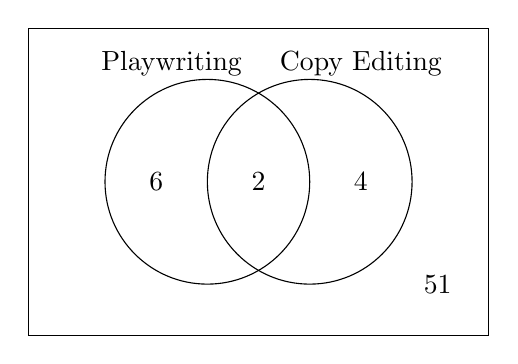
\begin{tikzpicture}[scale=0.65]
	\draw (0,0) rectangle (9,6);
	\draw (3.5,3) circle (2);
	\draw (5.5,3) circle (2);
	
	\node at (2.8,5.3) {Playwriting};
	\node at (6.5,5.3) {Copy Editing}; 
	
	\node at (2.5,3) {6};
	\node at (4.5,3) {2};
	\node at (6.5,3) {4};
	\node at (8,1) {51};
	\end{tikzpicture}
	\]
}



% Question 4
\newpage
\question[10] Not all people that work in the public sector have a college degree. Approximately 42\% of students go to college. Of those people that go to college, approximately 14\% work in the public sector while 22\% of non-college educated people work in the public sector. 
	\begin{enumerate}[(a)]
	\item What percent of people work in the public sector?
	\item What percent of people work in the public sector or go to college?
	\item If a person works in the public sector, what is the probability they hold a college degree?
	\end{enumerate} \pspace

{\itshape
\sol 
\begin{enumerate}[(a)]
\item 
	\[
	P(\text{Public})= 0.0588 + 0.1276= 0.1864
	\] \pspace

\item 
	\[
	P(\text{Public or College})= 0.0588 + 0.3612 + 0.1276= 0.5476
	\] \pspace

\item 
	\[
	P(\text{College} \;|\; \text{Public})= \dfrac{P(\text{College and Public})}{P(\text{Public})}= \dfrac{0.0588}{0.0588 + 0.1276}= \dfrac{0.0588}{0.1864}= 0.3155
	\]
\end{enumerate} \vfill
		\[
		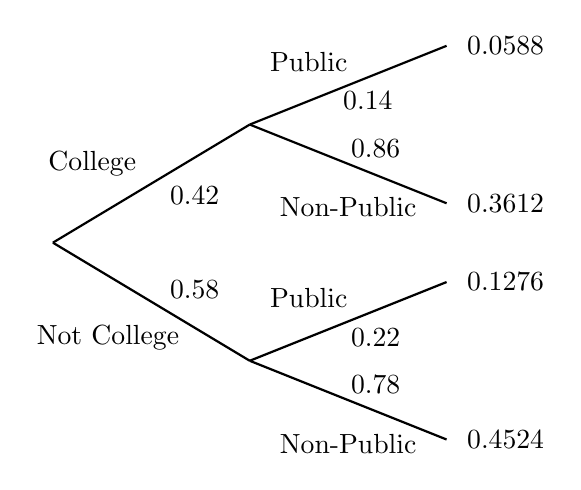
\begin{tikzpicture}[scale= 1.0]
		\def\FirstUpLabel{College}
		\def\FirstDownLabel{Not College}
		\def\SecondUpLabel{Public}
		\def\SecondDownLabel{Non-Public}
		\def\Up{$0.42$}
		\def\Down{$0.58$}
		\def\UpUp{$0.14$}
		\def\UpDown{$0.86$}
		\def\DownUp{$0.22$}
		\def\DownDown{$0.78$}
		\def\first{$0.0588$}
		\def\second{$0.3612$}
		\def\third{$0.1276$}
		\def\fourth{$0.4524$}
		
		\node at (0.5,1) {\FirstUpLabel};	
		\node at (0.7,-1.2) {\FirstDownLabel};	
		\node at (1.8,0.6) {\Up};
		\node at (1.8,-0.6) {\Down};
		\draw[thick] (0,0) -- (2.5,1.5);
		\draw[thick] (0,0) -- (2.5,-1.5);
		
		\node at (3.25,2.3) {\SecondUpLabel};
		\node at (3.75,0.45) {\SecondDownLabel};
		\node at (4,1.8) {\UpUp};
		\node at (4.1,1.2) {\UpDown};
		\node at (5.75,2.5) {\first};
		\node at (5.75,0.5) {\second};
		\draw[thick] (2.5,1.5) -- (5,2.5);
		\draw[thick] (2.5,1.5) -- (5,0.5);

		\node at (3.25,-0.7) {\SecondUpLabel};
		\node at (3.75,-2.55) {\SecondDownLabel};
		\node at (4.1,-1.2) {\DownUp};
		\node at (4.1,-1.8) {\DownDown};
		\node at (5.75,-0.5) {\third};	
		\node at (5.75,-2.5) {\fourth};	
		\draw[thick] (2.5,-1.5) -- (5,-0.5);
		\draw[thick] (2.5,-1.5) -- (5,-2.5);
		\end{tikzpicture}
		\]
}



% Question 5
\newpage
\question[10] A local casino sells a special `in-house' scratch ticket for \$1 that primarily offers discounts for various offerings around the hotel. However, there is a 1 in 500,000 chance to win \$100,000 and a 1 in 1,000 chance to win \$100. Find the expected net payout buying these scratch tickets. Is the sale of tickets for the casino a `wise' financial decision? \pspace

{\itshape
\sol From the casino's perspective, they earn \$1 each time they sell a ticket. If a player wins \$100, the casino only loses a net of \$99. If the player wins \$100,000, the casino only loses a net of \$99,999. The probability that a player does not win anything is $1 - \frac{1}{500000} - \frac{1}{1000}= \frac{499499}{500000}$ (assuming they cannot both win \$100,000 and \$100 simultaneously). The chart below then indicates the different casino net gains (with their probabilities) based on what (if anything) a player wins.
	\begin{table}[!ht] \renewcommand*{\arraystretch}{2.5}
	\centering
	\begin{tabular}{|l||c|c|c|} \hline
	Player Win & $\$0$ & $\$100$ & $\$100,000$ \\ \hline
	Probability & $\dfrac{499499}{500000}$ & $\dfrac{1}{1000}$ & $\dfrac{1}{500000}$ \\ \hline
	Casino Net Gain & $\$1$ & $-\$100$ & $-\$100,000$ \\ \hline
	\end{tabular}
	\end{table}
But then the expected value for the casino for these scratch tickets is\dots
	\[
	\begin{aligned}
	EX&= \sum x P(X= x) \\[0.3cm]
	&= \$1 \cdot \dfrac{499499}{500000} + (-\$100) \cdot \dfrac{1}{1000} + (-\$100000) \cdot \dfrac{1}{500000} \\[0.3cm]
	&= \$1 (0.998998) - \$100 (0.1) - \$100000(0.000002) \\[0.3cm]
	&= \$0.998998 - \$10 - \$0.2 \\[0.3cm]
	&\approx -\$8.80
	\end{aligned}
	\]
No, the sale of these tickets is not a `wise' financial decision for the casino. Because the expected value is $-\$8.80$, on average, the casino is losing an average of \$8.80 per ticket sale. If they wanted to turn a profit on the sale of these tickets, they should either change the probability of the player winning, lower the prize amounts, or increase the price of the scratch ticket. 
}



% Question 6
\newpage
\question[15] Data Science is one of the `hottest' fields of the last 15~years. The average salary for a data scientist is \$137,000. Suppose that these salaries are normally distributed with standard deviation \$39,000. 
	\begin{enumerate}[(a)]
	\item Find the percentage of data scientists that make less than \$100,000 per year.
	\item Find the percentage of data scientists that make more than \$100,000 per year.
	\item Find the probability that if you take a random sample of 5~data scientists that their average salary is less than \$100,000.  
	\end{enumerate} \pspace

{\itshape
\sol The distribution of data scientists' salaries is $N(\$137000, \$39000)$. 
\begin{enumerate}[(a)]
\item We have\dots
	\[
	z_{\$100K}= \dfrac{\$100000 - \$137000}{\$39000}= \dfrac{-\$37000}{\phantom{-}\$39000} \approx -0.95 \squiggle 0.1711
	\]
But then only 17.11\% of data scientists make less than \$100,000 per year. \pspace

\item We have\dots
	\[
	P(X > \$100K)= 1 - P(X < \$100K)= 1 - 0.1711= 0.8289
	\]
Therefore, 82.89\% of data scientists make more than \$100,000 per year. \pspace

\item To compute probabilities involving sample averages, we need to use the sampling distribution. For this, the Central Limit Theorem needs to apply. While the sample size of $n= 5$ is not sufficiently large, the underlying distribution is normal so that the Central Limit Theorem applies. By the Central Limit Theorem, the distribution of sample averages is normally distributed with distribution $N(\mu, \sigma/\sqrt{n})= N(\$137000, \$39000/\sqrt{5})= N(\$137000, \$17441.33)$. But then we have\dots
	\[
	z_{\$100K}= \dfrac{\$100000 - \$137000}{\$17441.33}= \dfrac{-\$37000}{\$17441.33}= -2.12 \squiggle 0.0170
	\]
Therefore, the probability of finding a random sample of 5~data scientists whose average salary is less than \$100,000 is 0.0170, i.e. 1.7\%
\end{enumerate}
}



% Question 7
\newpage
\question[10] A dual liberal arts college and conservatory accepts approximately 4,000 students each year. Of these students, approximately 15\% of these accepted students are admitted into the conservatory. You take a simple random sample of 13~students.
	\begin{enumerate}[(a)]
	\item Find the probability that at most 4 of these students were admitted to the conservatory. 
	\item Find the probability that more than 5 of these students were admitted to the conservatory. 
	\item Find the probability that at least one of these students was admitted to the conservatory. 
	\end{enumerate} 

{\itshape 
\sol Each student is either accepted or not. We assume that the probability that any student is accepted is 15\%, i.e. the probability of acceptance is $p= 0.15$. We take a fixed sample of $n= 13$ students, which we assume is chosen independently. Therefore, this is a binomial distribution with $n= 13$ and $p= 0.15$, i.e. $B(13, 0.15)$. We let $X$ represent the number of students in the sample that are admitted. 

\begin{enumerate}[(a)]
\item We have\dots
	\[
	\begin{aligned}
	P(X \leq 4)&= P(X= 0) + P(X= 1) + P(X= 2) + P(X= 3) + P(X= 4) \\[0.1cm]
	&\approx 0.1209 + 0.2774 + 0.2937 + 0.1900 + 0.0838 \\[0.1cm]
	&= 0.9658
	\end{aligned}
	\]
Therefore, there is a 96.58\% chance that at most 4 of the 13 students were admitted to the conservatory. 

\item We have\dots
	\[
	\begin{aligned}
	P(X > 5)&= P(X= 6) + P(X= 7) + \cdots + P(X= 13) \\[0.1cm]
	&= 1 - \left( P(X \leq 4) + P(X= 5) \right) \\[0.1cm]
	&\approx 1 - ( 0.9658 + 0.0266) \\[0.1cm]
	&= 1 - 0.9924 \\[0.3cm]
	&= 0.0076
	\end{aligned}
	\]
	\[ \text{\itshape OR} \]
	\[
	\begin{aligned}
	P(X > 5)&= P(X= 6) + P(X= 7) + \cdots + P(X= 13) \\[0.1cm]
	&\approx 0.0063 + 0.0011 + 0.0001 + 0.0000 + \cdots + 0.0000 \\[0.1cm]
	&= 0.0075
	\end{aligned}
	\]
Therefore, the probability that more than 5 of the 13 people were admitted is approximately 0.75\%. 

\item 
	\[
	P(X \geq 1)= P(X= 1) + P(X= 2) + \cdots + P(X= 13)= 1 - P(X= 0)= 1 - 0.1209= 0.8791
	\]
Therefore, the probability that at least one student from the 13 was admitted is 87.91\%.
\end{enumerate}
}



% Question 8
\newpage
\question[10] A medical researcher is examining the relation between vitamin levels in blood and cancer risks. Based on a sample of 200~cancer-free individuals, an average of 11.7~mg/L of a particular vitamin were found in patients blood. Assuming a standard deviation of $\sigma= 3.65 \text{ mg/L}$, find a 92\% confidence interval for the level of vitamin found in cancer-free blood. \pspace

{\itshape
\sol We have a same average of $\overline{x}= 11.7 \text{ mg/L}$ and a sample size of $n= 200$. We know that the standard deviation of the underlying population is $\sigma= 3.65 \text{ mg/L}$. Because the sample size of $n= 200 > 30$ is `sufficiently large', the Central Limit Theorem applies. But then the confidence interval will be given by $\overline{x} \pm z^*\, \frac{\sigma}{\sqrt{n}}$, where $z^*$ is the $z$-value corresponding to a 92\% confidence interval. \par
	\[
	\begin{tikzpicture}[scale=1.2,every node/.style={scale=0.5}]
	\begin{axis}[
%	grid=both,
	axis lines=middle,
	ticklabel style={fill=blue!5!white},
	axis y line= none,
	axis x line=none,
	xmin= -10.5, xmax=10.5,
	ymin= -0.5, ymax=0.5,
	xtick={-10,-8,...,10},
	ytick={-10,-8,...,10},
	minor x tick num = 1,
	minor y tick num = 1,
%	xlabel=\(x\),ylabel=\(y\),
	]
	\addplot[line width=0.03cm,domain=-4:4,samples=100] {gauss(0,1)};
	\draw[line width=0.03cm] (-6,-0.02) -- (6,-0.02);
	\draw[line width=0.03cm,dotted] (-2,-0.02) -- (-2,0.053991);
	\draw[line width=0.03cm,dotted] (2,-0.02) -- (2,0.053991);
	\end{axis}
	\end{tikzpicture}
	\] \par
If `92\% of the possible values' are in this interval, that leaves 8\% for `each end' of the distribution. By symmetry, this leaves 4\% of values in the `lower left' end of this distribution. But then $92\% + 4\%= 96\%$ of values are to the left of the upper value in the confidence interval. But then this value has a $z$-score corresponding to $0.96$, which implies $z^*$ corresponds to $0.96$. But then we know that $z^* \approx 1.75$. But then we have\dots
	\[
	\begin{aligned}
	\overline{x} - z^*\, \dfrac{\sigma}{\sqrt{n}}&= 11.7 - 1.75 \cdot \dfrac{3.65}{\sqrt{200}} \approx 11.7 - 0.452= 11.248 \text{ mg/L} \\[0.3cm]
	\overline{x} + z^*\, \dfrac{\sigma}{\sqrt{n}}&= 11.7 + 1.75 \cdot \dfrac{3.65}{\sqrt{200}} \approx 11.7 + 0.452= 12.152 \text{ mg/L}
	\end{aligned}
	\]
But then there is a 92\% interval is $(11.248 \text{ mg/L}, 12.152 \text{ mg/L})$. 
}



% Question 9
\newpage
\question[10] An architect is working on plans for an academic building. For a large lecture hall, the architect is trying to determine how many left handed sets should be placed in the room. The lecture hall will have 250~seats. Research suggests that approximately 11\% of individuals are left-handed. The architect decides to place 35 left handed seats in the room. Use the normal approximation to find the probability that if the lecture hall is full that there will be at most 35 left handed students in the room. \pspace

{\itshape
\sol Each student is either left-handed or not and we assume the probability that a person is left-handed is 11\%. There will be a maximum fixed number of 250 `observations', i.e. maximum people that can be seated in the room. We assume the `handedness' of the individuals seated in the room is independent. But then this is a binomial distribution with $n= 250$ and $p= 0.11$, i.e. $B(250, 0.11)$. But because $np= 250 (0.11)= 27.5 \geq 10$ and $n(1 - p)= 250(1 - 0.11)= 250(0.89)= 222.5 \geq 10$, the Central Limit Theorem applies. Therefore, we can use the normal approximation to the binomial distribution. The binomial distribution for counts is $B(n, p) \approx N(np, \sqrt{np(1 - p)} )$. But we have\dots
	\[
	\hspace{-0.5cm} N\big(np, \sqrt{np(1 - p)} \big)= N\big( 250 \cdot 0.11, \sqrt{250 \cdot 0.11 (1 - 0.11)} \big)= N\big(27.5, \sqrt{24.475} \big)= N(27.5, 4.947)
	\]
Letting $X$ be the number of left-handed people in the room, we need to find $P(X \leq 35)$. But we have\dots
	\[
	z_35= \dfrac{x - \mu}{\sigma}= \dfrac{35 - 27.5}{4.947}= \dfrac{7.5}{4.947} \approx 1.52 \squiggle 0.9357
	\]
But then we know that $P(X \leq 35)= 0.9357$, i.e. there is a 93.57\% chance that when the room is full, there will be enough left-handed seats for the left-handed people in the room. 
}


\end{questions}
\end{document}